\documentclass{article}
\usepackage[a4paper,left=3cm,right=3cm,top=3cm,bottom=3cm]{geometry}
\usepackage[utf8]{inputenc}
\usepackage[T1]{fontenc}
\usepackage{latexsym,amsfonts,amsmath,amssymb,amstext,graphicx,titlesec,ae,aecompl,mathtools,tabularx, multirow, cancel, nicefrac,subcaption, blindtext, floatrow}
\setlength{\parindent}{0pt}
\newfloatcommand{capbtabbox}{table}[][\FBwidth]


\begin{document}

\begin{titlepage}
       \begin{center}
             \begin{huge}
				   %% Update assignment number here
                   \textbf{Assignment 4}
             \end{huge}
       \end{center}

       \begin{center}
             \begin{large}
                   Computational Intelligence, SS2020
             \end{large}
       \end{center}

       \begin{center}
 \begin{tabularx}{\textwidth}{|>{\hsize=.33\hsize}X|>{\hsize=.33\hsize}X|>{\hsize=.33\hsize}X|} 

                   \hline
                   \multicolumn{3}{|c|}{\textbf{Team Members}} \\
                   \hline
                   Last name & First name & Matriculation Number \\
                   \hline
                   Blöcher & Christian & 01573246 \\
                   \hline
                   Bürgener & Max & 01531577 \\
                   \hline
                    &  &  \\
                   \hline

             \end{tabularx}
       \end{center}
\end{titlepage}


\section{Linear SVM}

\subsection{Plots}

\begin{figure}[!ht]
	\centering
	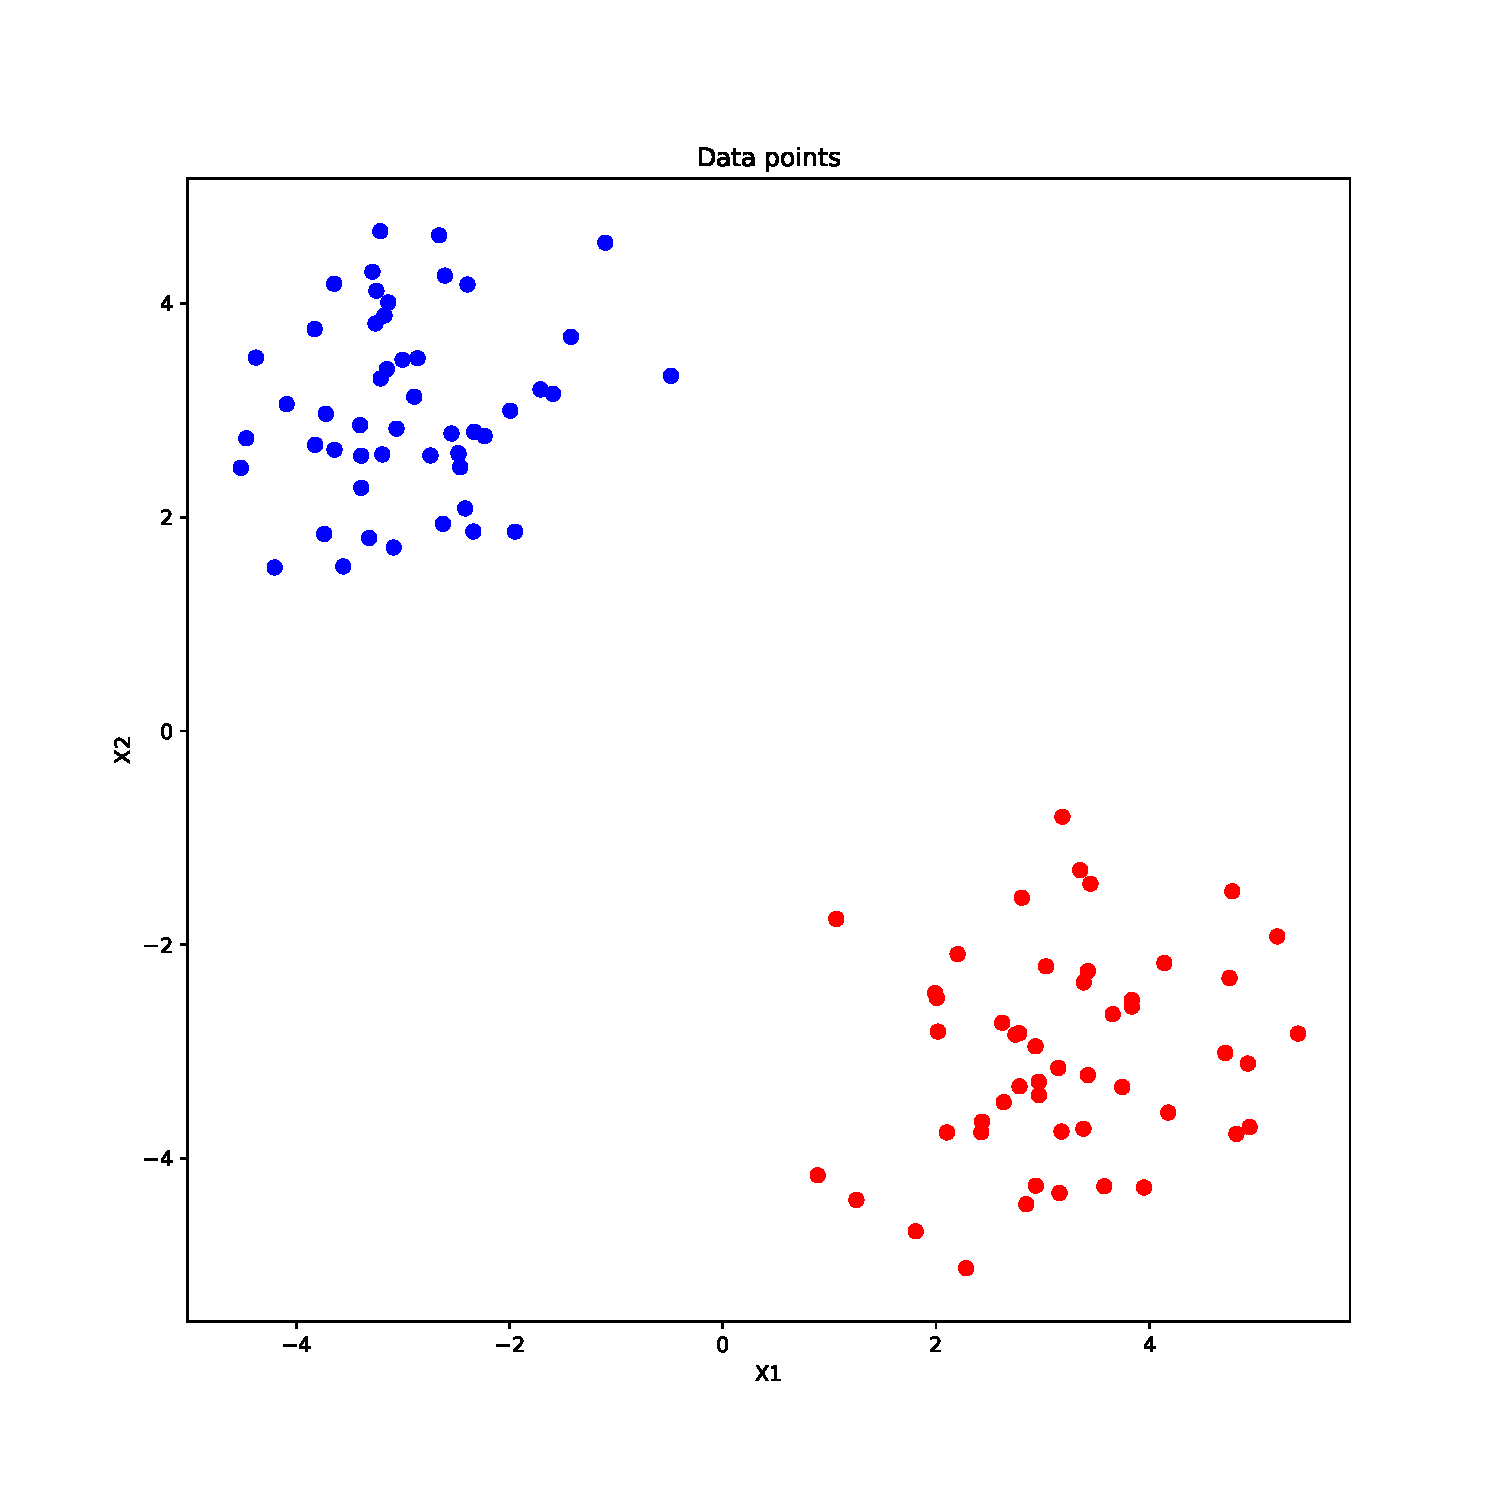
\includegraphics[width=.6\textwidth]{./Figures/1_data}
	\caption{Dataset}
	\label{Dataset}
\end{figure}

\begin{figure}[!ht]
	\makebox[\textwidth]{
	\begin{subfigure}{0.6\textwidth}
	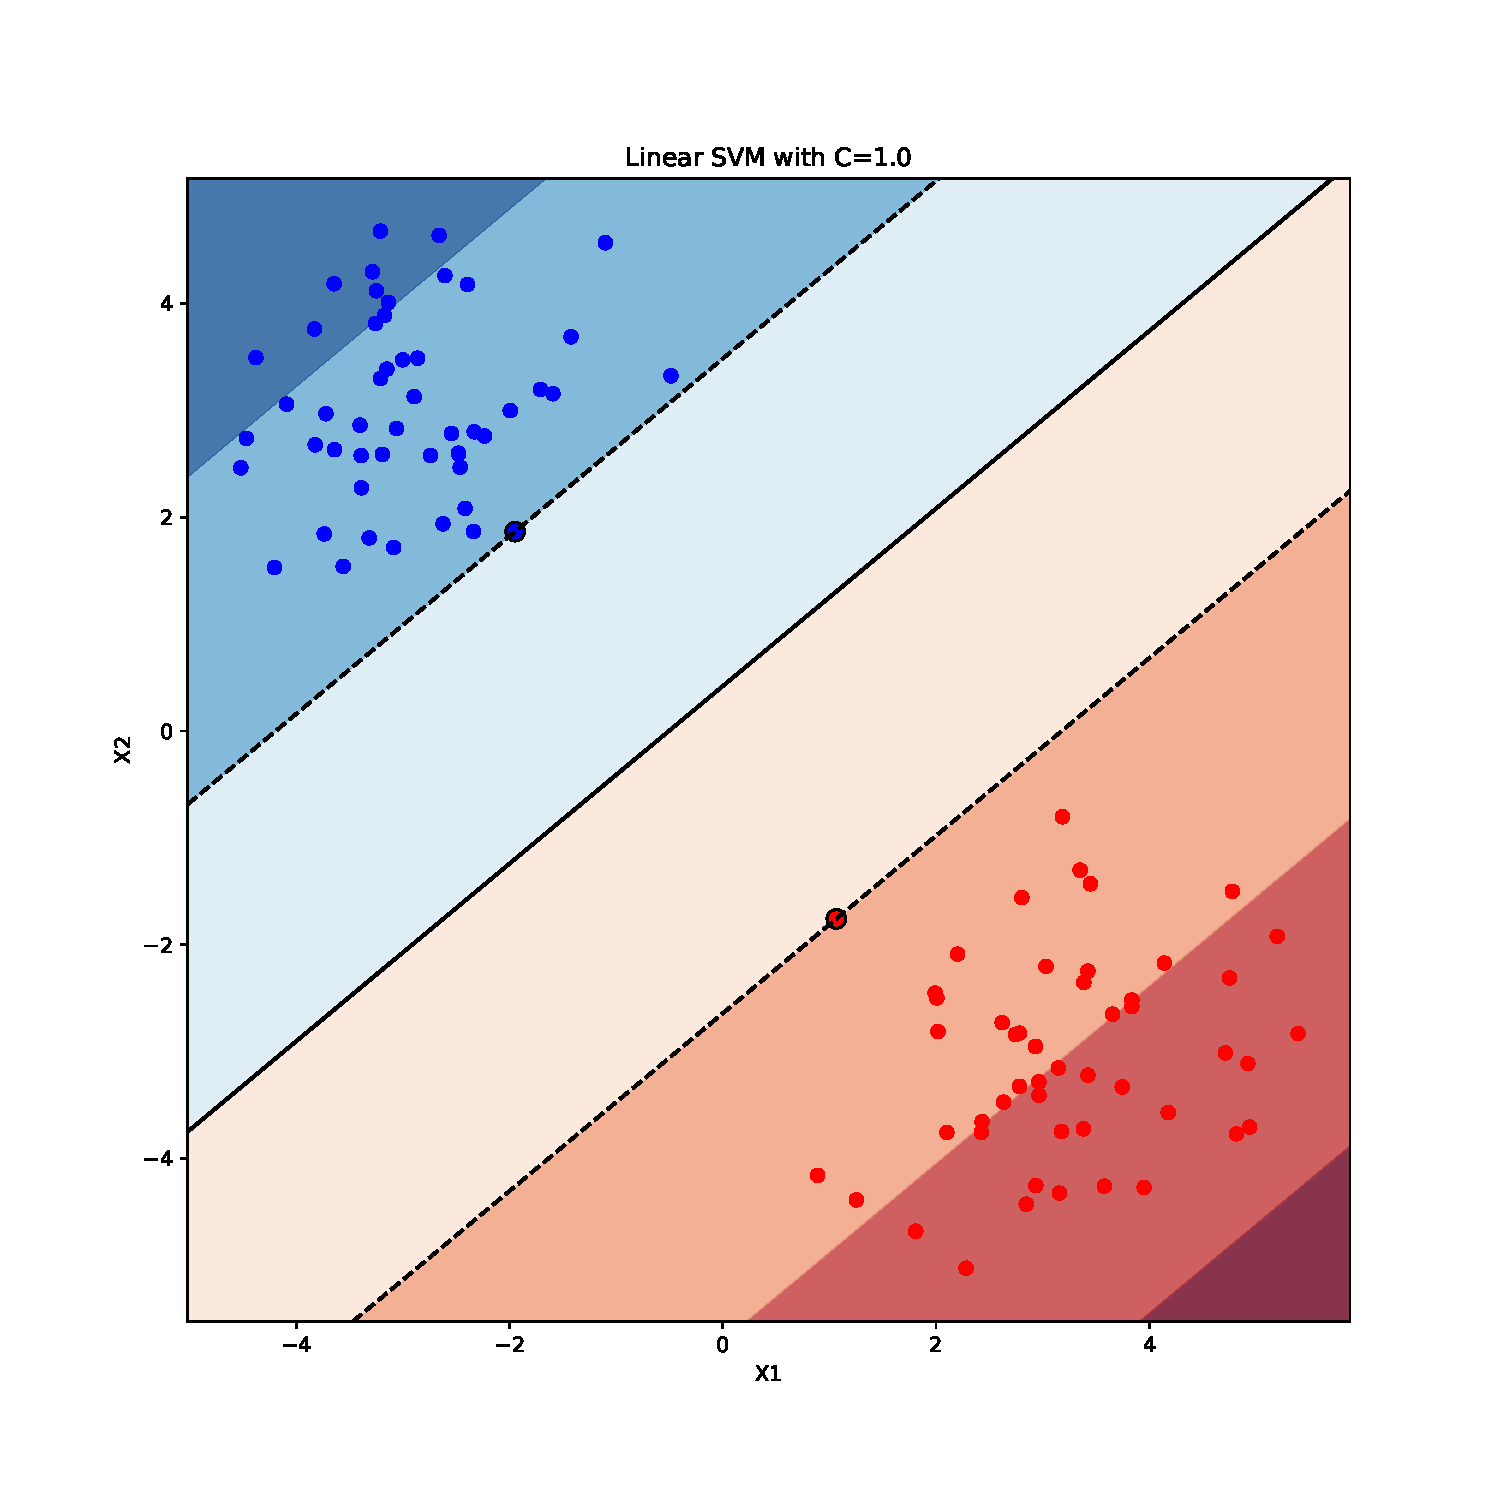
\includegraphics[width=\textwidth]{./Figures/1a_bound.pdf}
	\caption{Dataset}
	\end{subfigure}
	\begin{subfigure}{0.6\textwidth}
	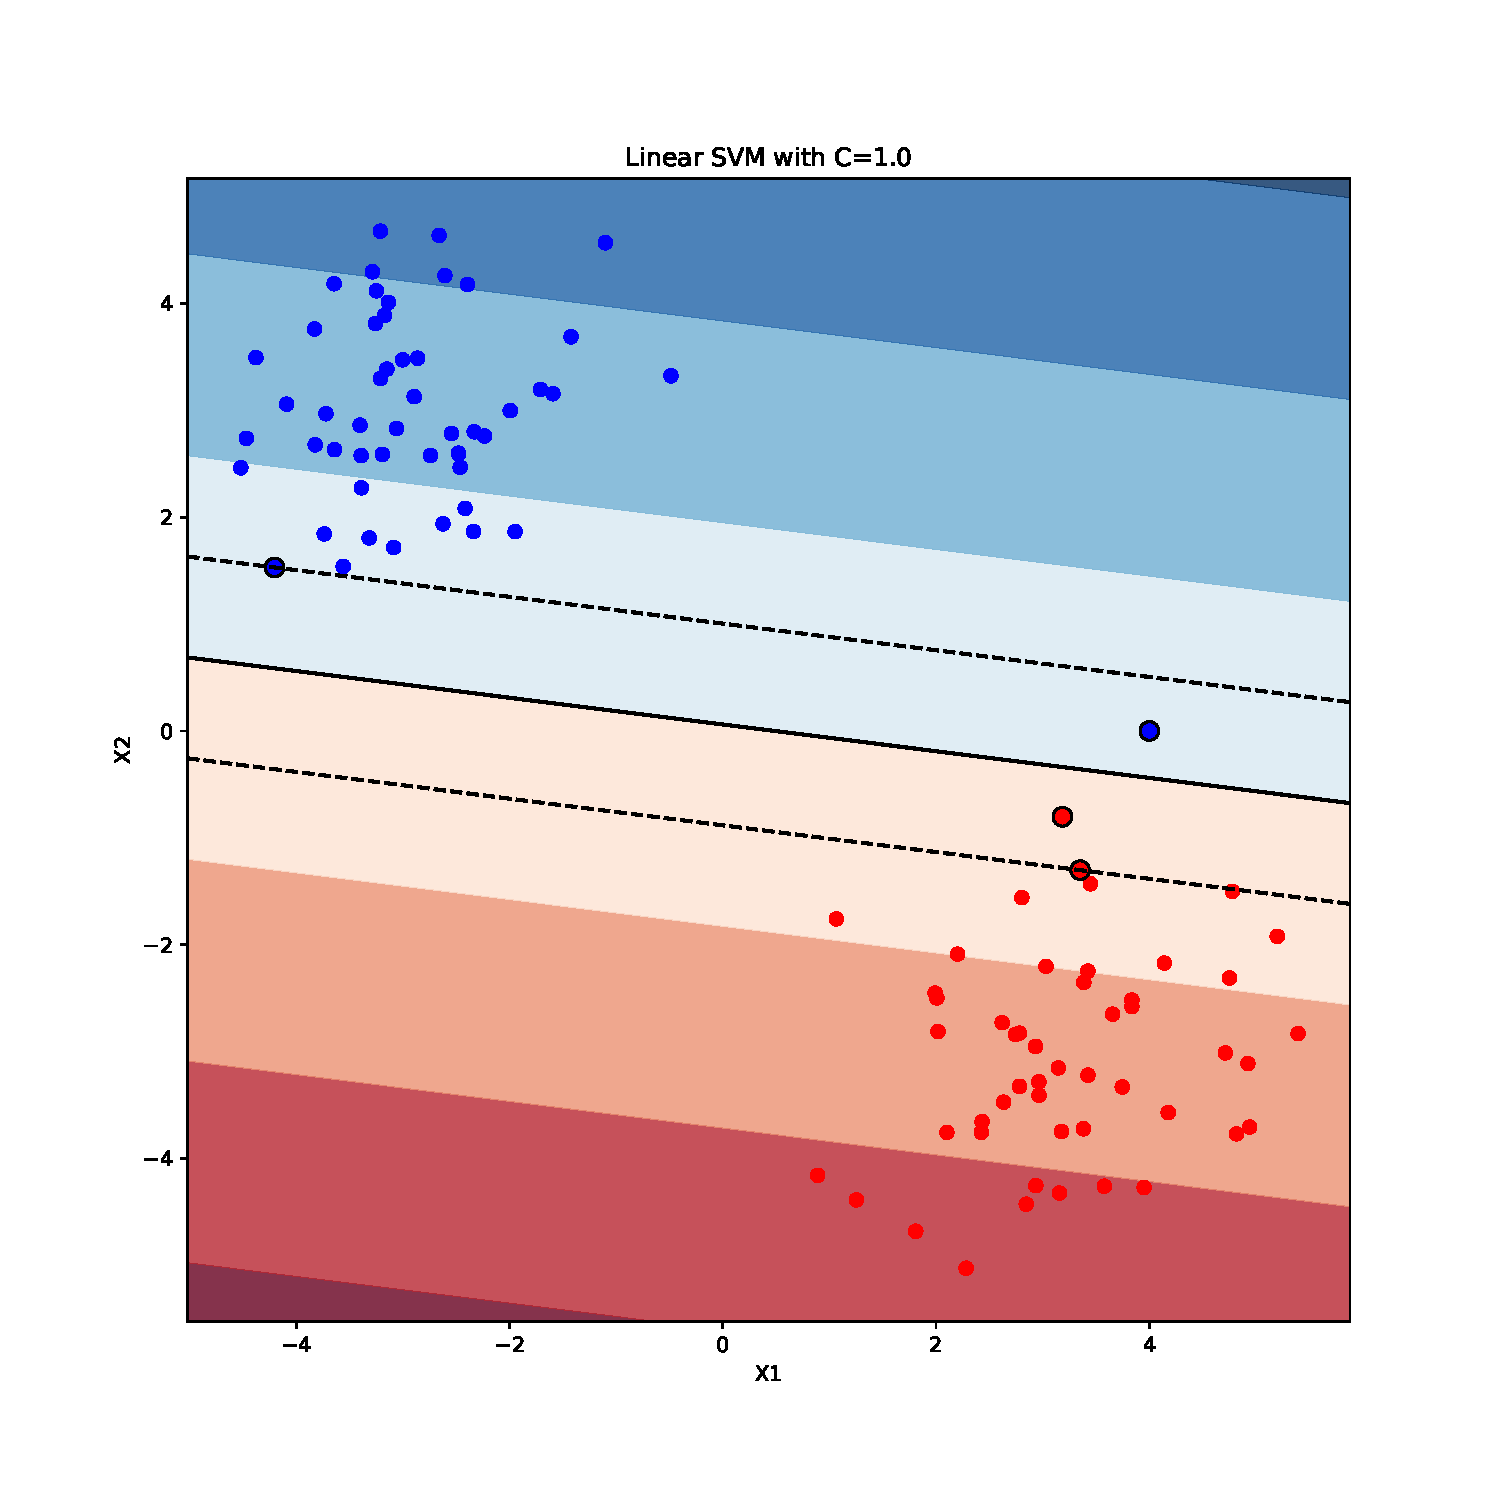
\includegraphics[width=\textwidth]{./Figures/1b_bound}
	\caption{Dataset with additional data point}
	\end{subfigure}
	}	
	\caption{Classification of the dataset using SVM}
	\label{SVM_classification}
\end{figure}

\begin{figure}[!ht]
    \centering
    \makebox[\textwidth]{
    \begin{subfigure}{0.6\textwidth}
    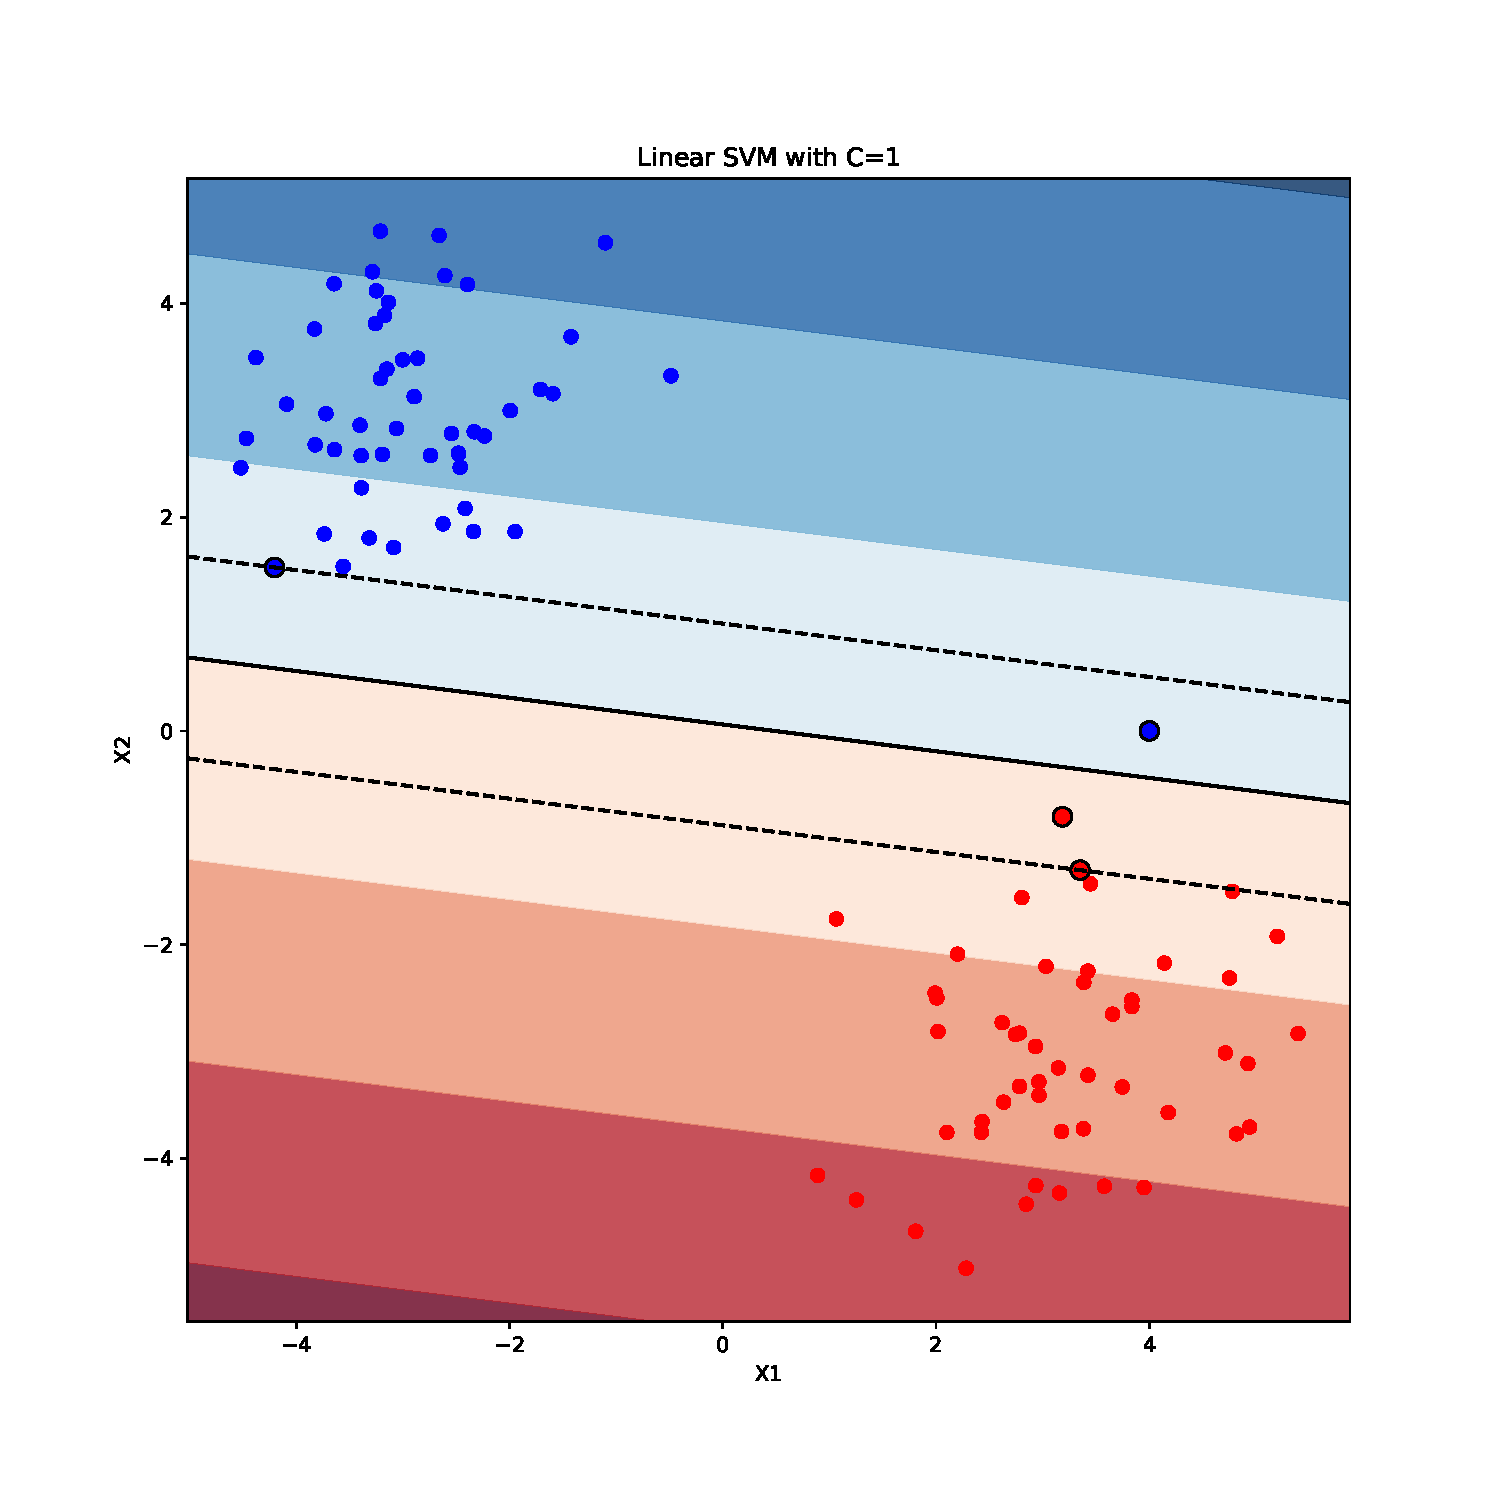
\includegraphics[width=\textwidth]{./Figures/1c_bound_C1.pdf}
    \caption{$C=1$}
    \end{subfigure}
    \begin{subfigure}{0.6\textwidth}
    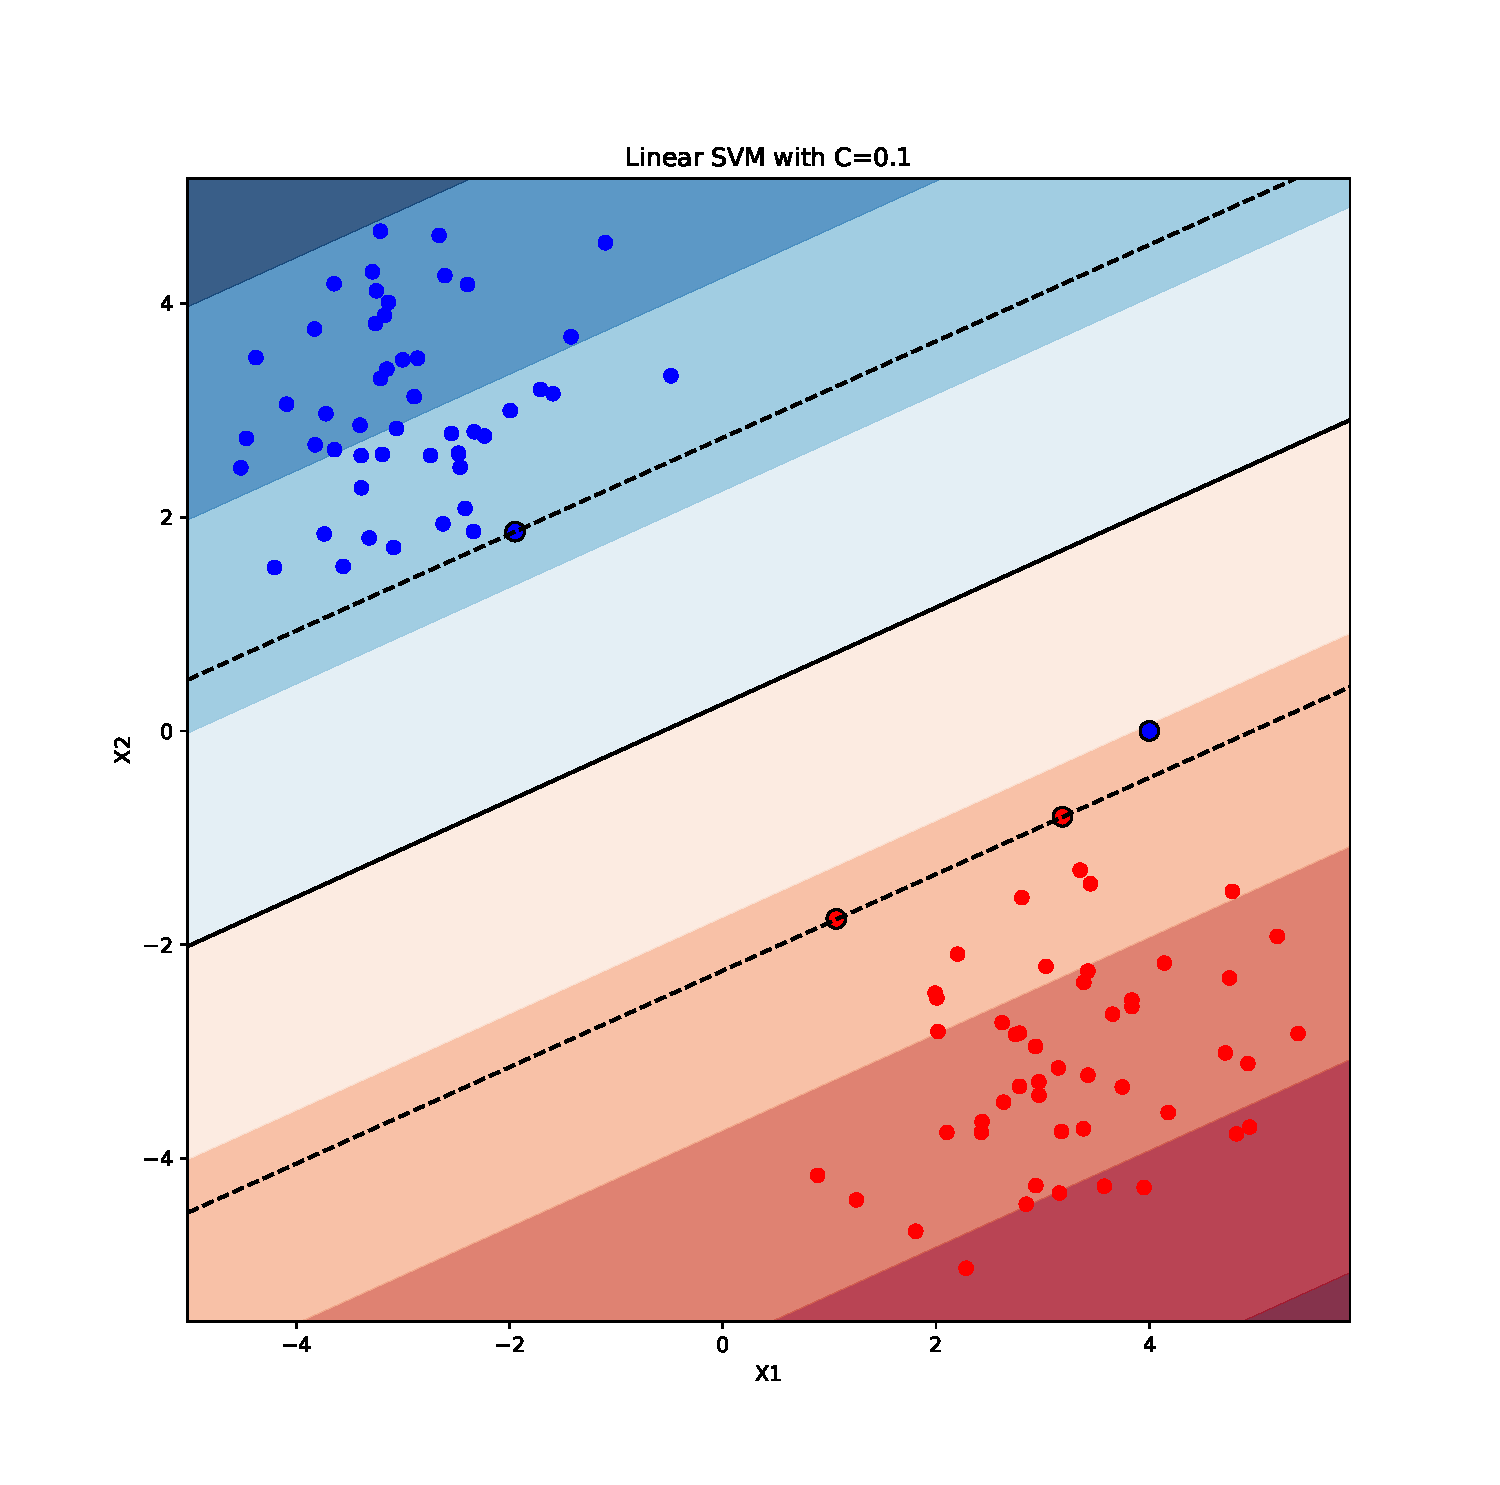
\includegraphics[width=\textwidth]{./Figures/1c_bound_C01.pdf}
    \caption{$C=0,1$}
    \end{subfigure}
    }
    
    \makebox[\textwidth]{
    \begin{subfigure}{0.6\textwidth}
    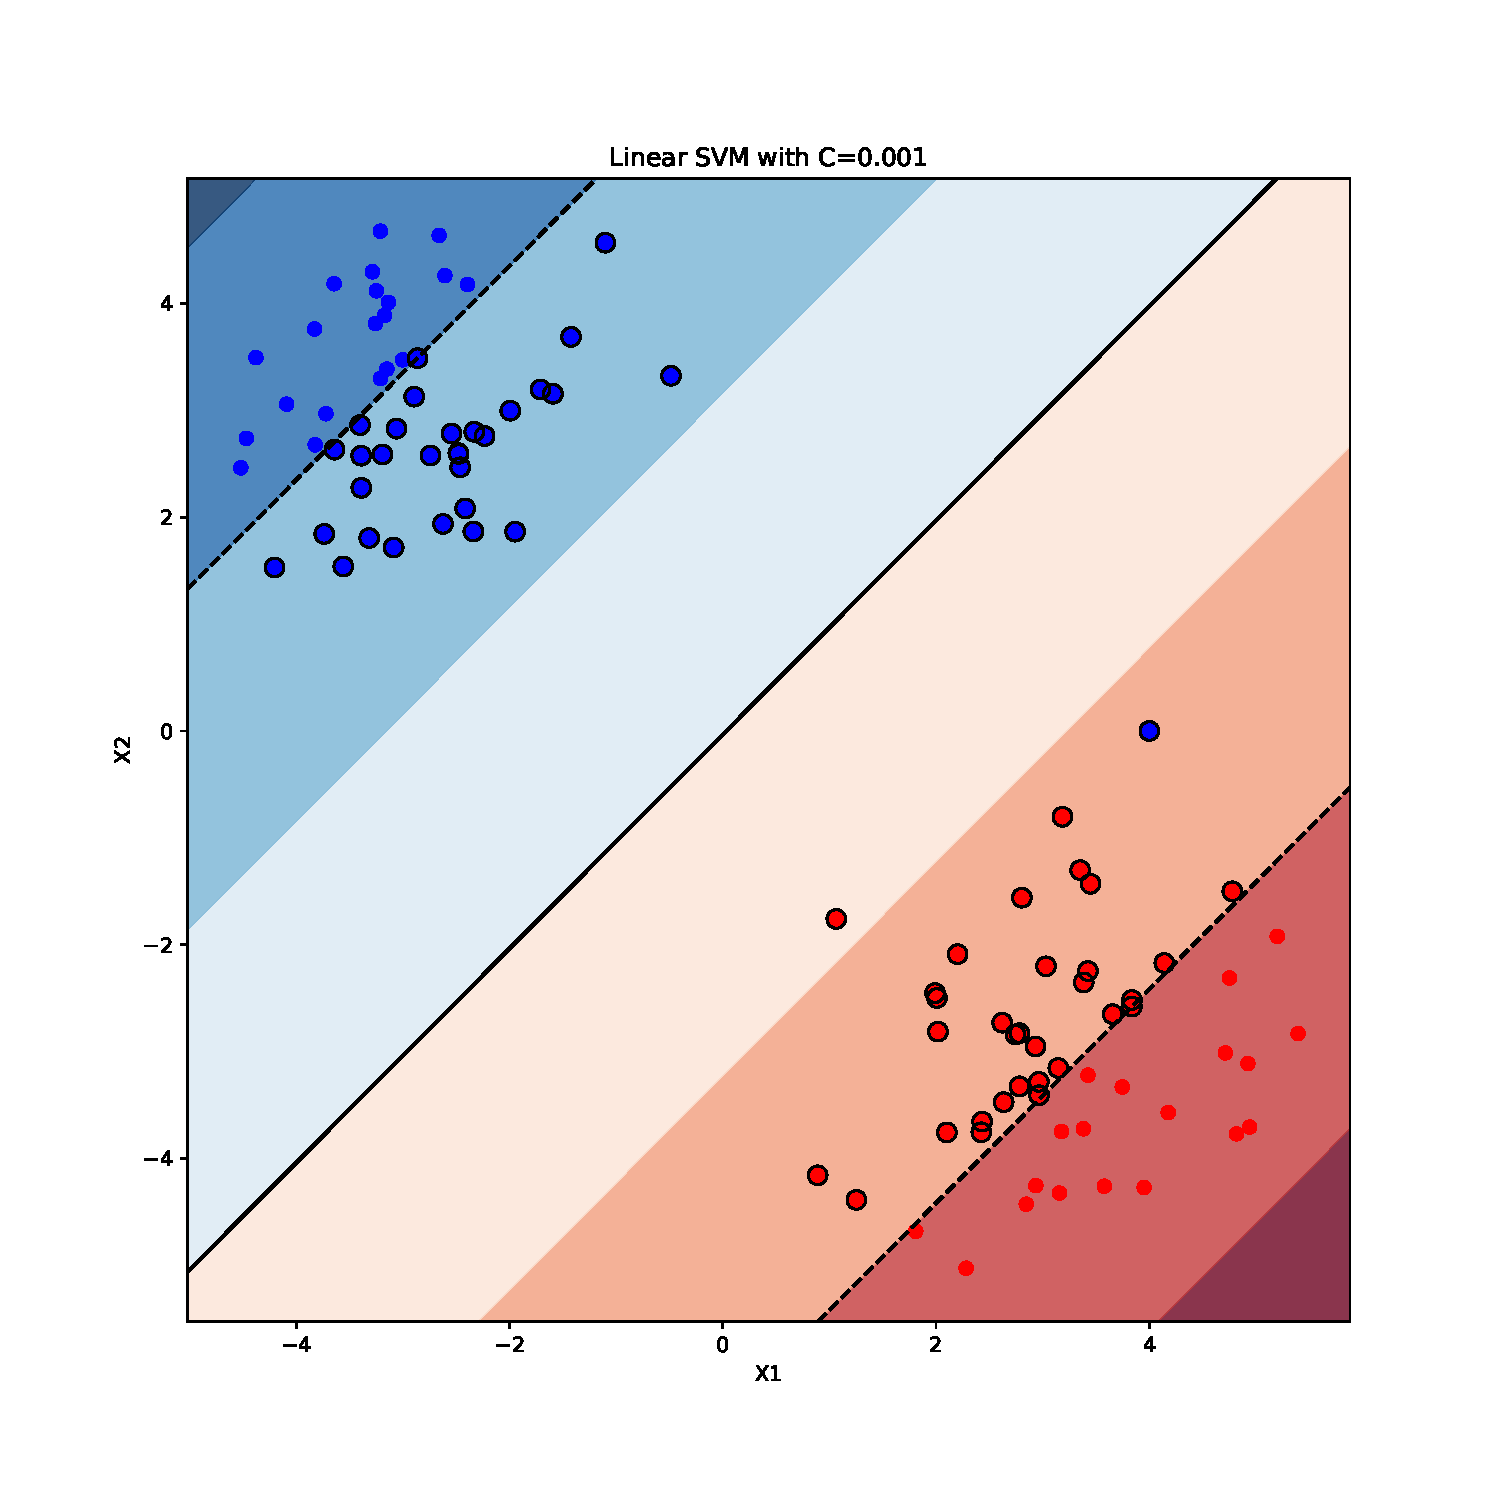
\includegraphics[width=\textwidth]{./Figures/1c_bound_C0001.pdf}
    \caption{$C=0,001$}
    \end{subfigure}
    \begin{subfigure}{0.6\textwidth}
    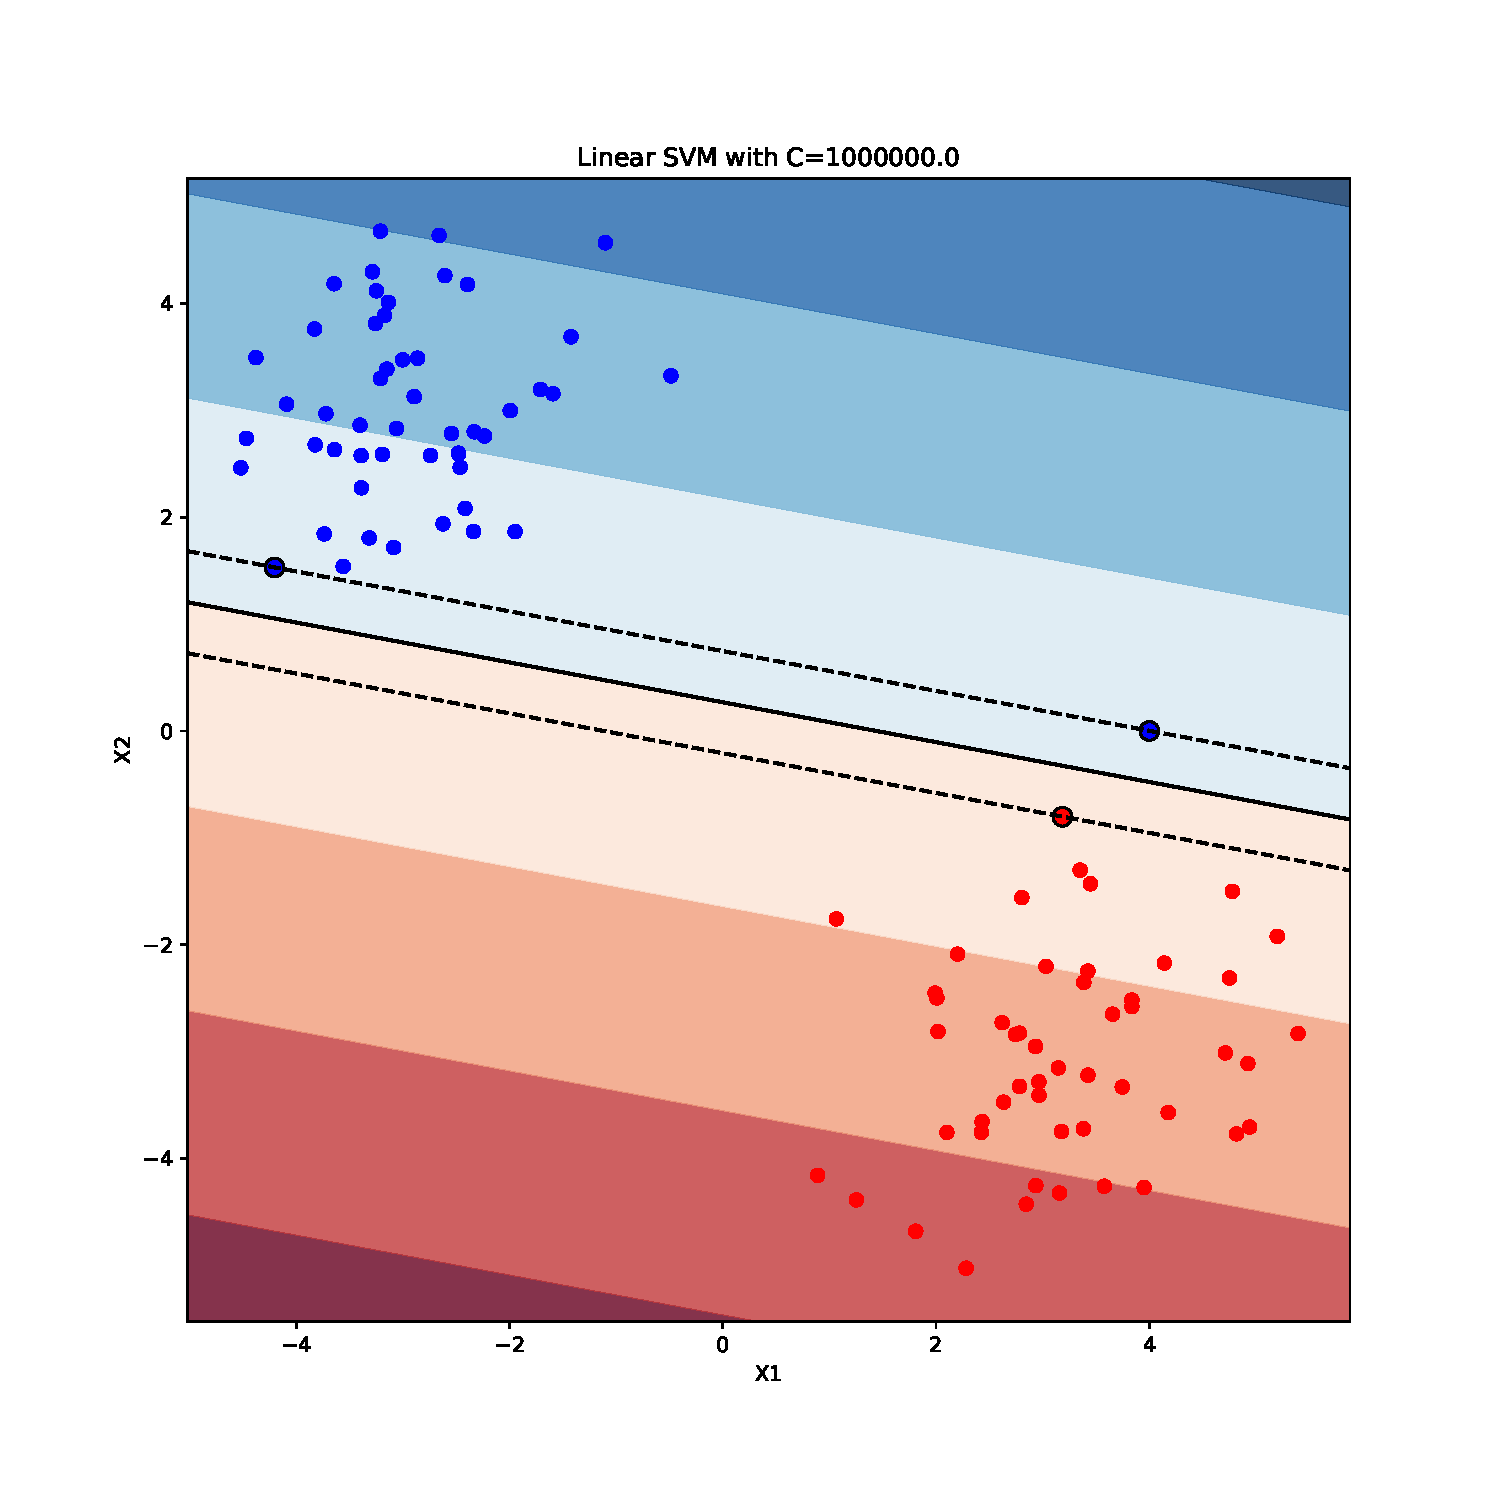
\includegraphics[width=\textwidth]{./Figures/1c_bound_C1e6.pdf}
    \caption{$C=1000000$}
    \end{subfigure}
    }
    \caption{SVM Classification using different C parameters}
    \label{SVM_Cs}
\end{figure}

\subsection{How and why changed the decision boundary when the new point was added?}

The margin is defined as the perpendicular distance between the decision boundary and the closest data point. Since the new added data point is located in the margin the algorithm adjusts its solution by choosing the option with the smallest generalization error. Apparently this solution includes more support vectors (data points within and on the margin boundary).

\subsection{The inverse regularization parameter $C$}

\begin{itemize}

	\item $C$ controls the penalization of data points within the margin. It is scaling data samples so that samples can be misclassified or lie within the margin boundary. This is helpful since not all problems can be clearly separated.

	\item Figure \ref{SVM_Cs} is showing the classification using different values for $C$. The margin boundary gets larger with decreasing values for $C$. As a result the classification is showing more support vectors and also misclassifies the additional data point since these points are less penalized.
	    A very large value for C leads to the strict constraint that the margin borders are denoting the closest data point to the decision boundary. Therefore the margin boundary is very small.

\end{itemize}


\section{Nonlinear (kernel) SVM}

\subsection{}

\subsection{}

\subsection{}

\subsection{}

\subsection{}


\section{Multiclass classification}

\subsection{'One vs. Rest' vs. 'One vs. All' algorithms}

SVMs are fundamentally two-class classifier. We can use different approaches to solve problems with $K$ classes. \\
The 'One vs. Rest' algorithm compares the to be determined class (positive) with the rest of the dataset (negative). During the scoring phase the algorithm determines the probability for each class of a sample using the binary classifiers.\\
'One vs. All' creates $K(K-1)/2$ classifiers, which means that we use all possible pairs of classes. Each binary classifiers predicts one class. For classification the class with the highest number of predictions will be chosen. That algorithm requires in comparison to the 'One vs. Rest approach' much more time to get trained and to classify.

\newpage

\subsection{Classification using linear and RBF}

\begin{figure}[!ht]
	\centering
	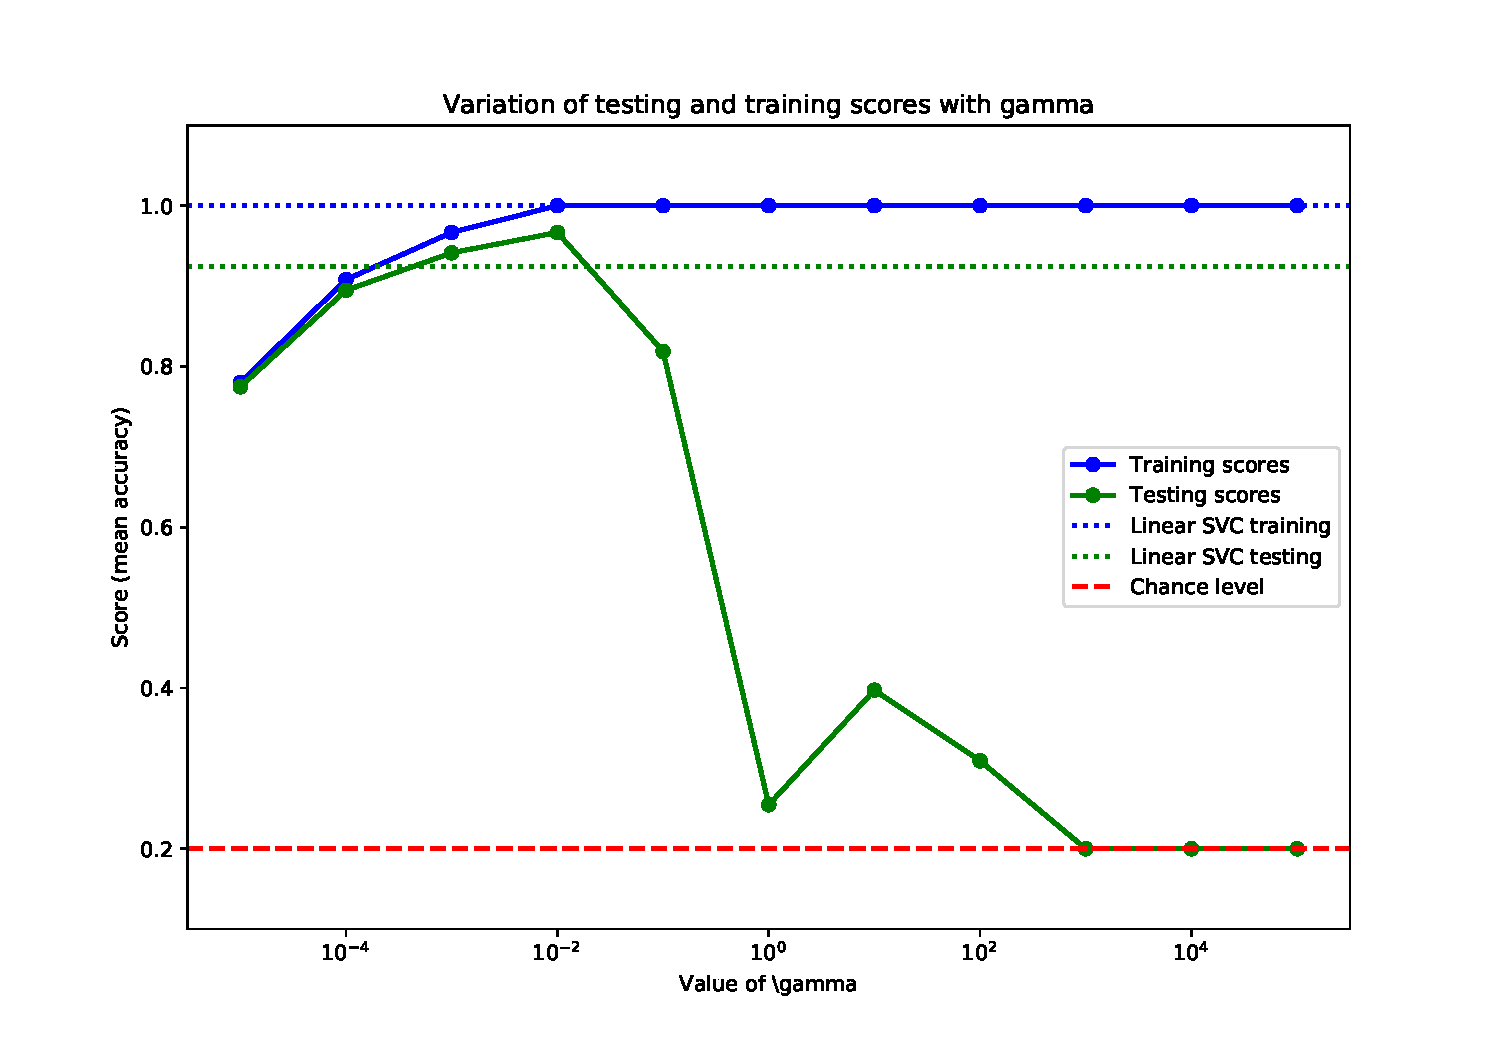
\includegraphics[width=.8\textwidth]{./Figures/3a_score.pdf}
	\caption{Scores using linear and RBF kernel on MNIST Dataset}
	\label{multiclass_classification}
\end{figure}

\begin{itemize}

	\item Figure \ref{multiclass_classification} shows that the linear kernel performs very well on MNIST image classification. Using $\gamma = 0,1$ the RBF classification performs slightly better than the linear kernel. For higher $\gamma$ values the classification overfits and the testing scores are quickly descending.
	
	\item The linear kernel performs good, because the sample features which are generated from the MNIST pictures must be very good linear separable in higher dimensions. 

\end{itemize}

\subsection{Confusion matrix}

    \begin{figure}[hbt!]
    \begin{floatrow}
    \ffigbox{%
    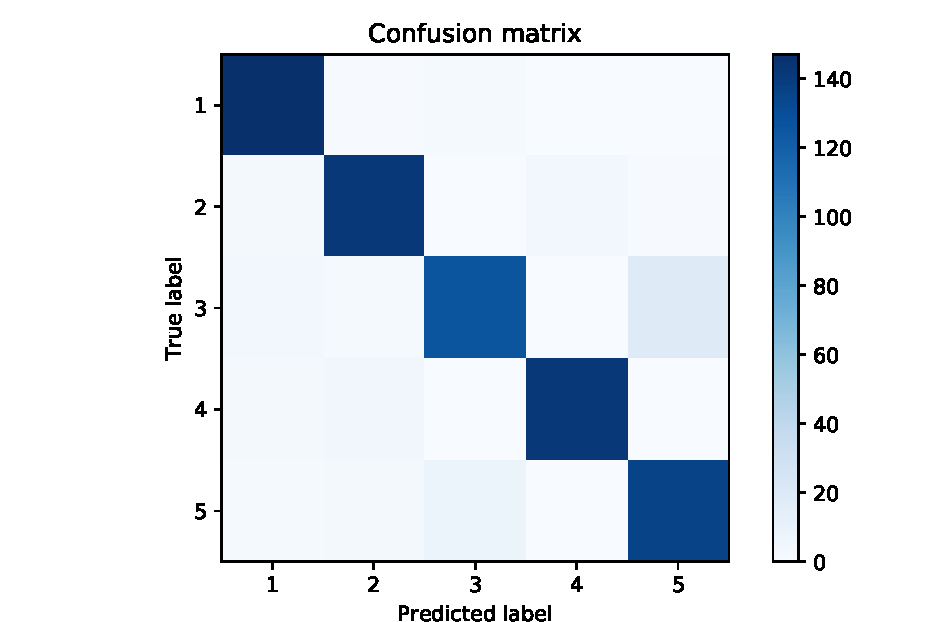
\includegraphics[width=.5\textwidth]{./Figures/3b_confusionmatrix.pdf}
    }{%
    \caption{Confusion matrix}%
    \label{confusion_matrix}
	}
	\capbtabbox{%
	\begin{tabular}{|l|l|l|l|l|l|}
	\hline
	  & 1   & 2   & 3   & 4   & 5   \\ \hline
	1 & 147 & 1   & 2   & 0   & 0   \\ \hline
	2 & 3   & 142 & 0   & 4   & 1   \\ \hline
	3 & 4   & 2   & 126 & 0   & 18  \\ \hline
	4 & 3   & 5   & 0   & 142 & 0   \\ \hline
	5 & 2   & 3   & 9   & 0   & 136 \\ \hline
	\end{tabular}
	}{%
	\caption{Confusion matrix}%
	}
	\end{floatrow}
	\end{figure}\\
	
The rows of our confusion matrix correspond to the true classes and the columns to the predicted classes. Class three is the most misclassified class with score of 84\%. 

\newpage

\subsection{Misclassified images}

\begin{figure}[!ht]
	\centering
	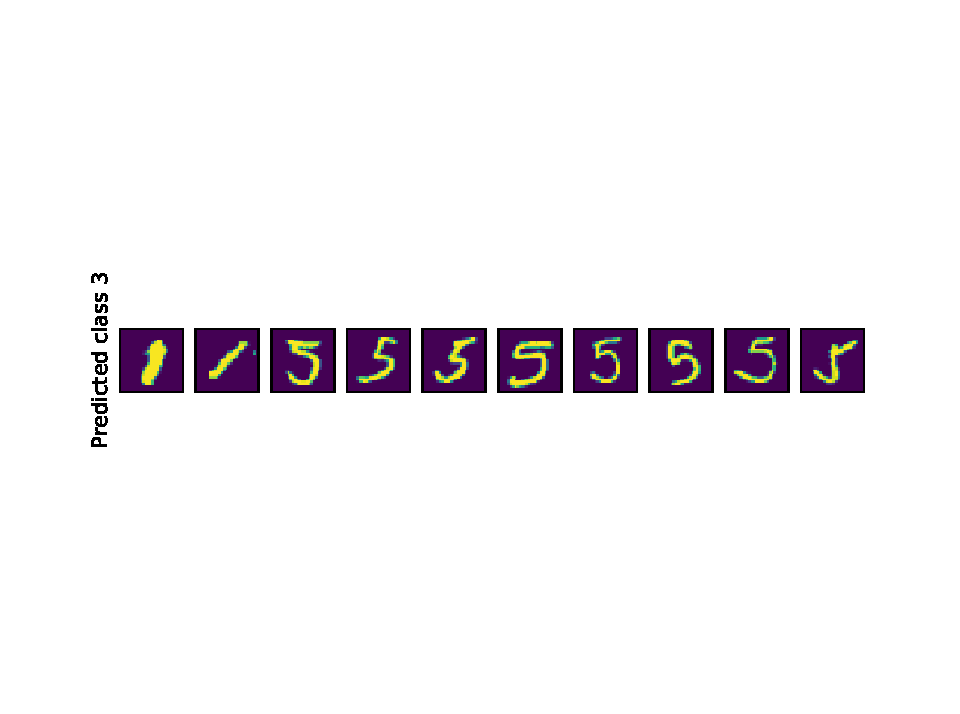
\includegraphics[width=\textwidth]{./Figures/3b_misclassifieditems.pdf}
	\caption{Misclassified images}
	\label{mnist_misclassified}
\end{figure}

Figure \ref{mnist_misclassified} shows the column of class three. The images are showing the real numbers, which were classified as class three. Apparently the algorithms has problems to distinguish threes and fives. Probably because the lower part of these numbers are very similar. The reason for both falsely determined ones could be that they are untypical ones. The first one is very bold and the other is a bit rotated.


\section{SVM with Gradient Descent}

\subsection{}

\subsection{}

\subsection{}

\subsection{}

\end{document}}